\documentclass[twocolumn]{article}
\usepackage{amsmath}
\usepackage{graphicx}
\graphicspath{documents/}
\usepackage{caption}
\captionsetup{font=scriptsize}
\usepackage[margin=0.5in]{geometry}
\usepackage{float}

\title{Statistics, Uncertainties and Linear Fitting}
\author{Jorge A. Garcia}
\date{February 6th, 2018\\\line(1,0){500}}

\begin{document}
\maketitle

\section{Machine Numbers}

A great resource that helped with this problem is the ''IEEE-754 Floating Point Converter'' by Schmidt, which can be found in the web. It allows to see the binary
conversion of a number and even the error associated due to conversion (although this error probably should be taken with a grain of salt, since it itself is a product
from a numerical computation).

Entering 0.0078125, the number can be represented as $1\times2^{-7}$, so it can be represented exactly on a computer. It requires only a value for the exponent, since
the mantissa has always as given the value of $1*2^0$. This is what is called a machine number \cite{hjorth}. Its binary representation in a 32-bit machine is then:
\begin{equation*}
 |0|01111000|00000000000000000000000|
\end{equation*}
Which is divided into $|sign|exponent|mantissa|$.

The number $0.2$ on the other hand is not a linear combination of powers of 2, so it can not be represented exactly. It's then approximated with an error of roughly
$3^{-9}$. It's binary representation is then:
\begin{equation*}
  |0|01111100|10011001100110011001101|
\end{equation*}


\section{Hermite Polynomials}

In order to recreate the mathematical expressions for the first 5 Hermite polynomials, a Python module named SymPy was used. It functions similarly to the symbolic
manipulation in MATLAB. Using a loop to determine the order of the derivative, Figure \ref{fig:hexp} shows the generated functions plotted from $[-3,3]$.
\begin{align*}
 H_0 &= 1 \\
 H_1 &= 2x \\
 H_2 &= 4x^2-2 \\
 H_3 &= 8x^3 - 12x \\
 H_4 &= 16x^4 - 48x^2 + 12
\end{align*}

\begin{figure}[h!]
  \centering
  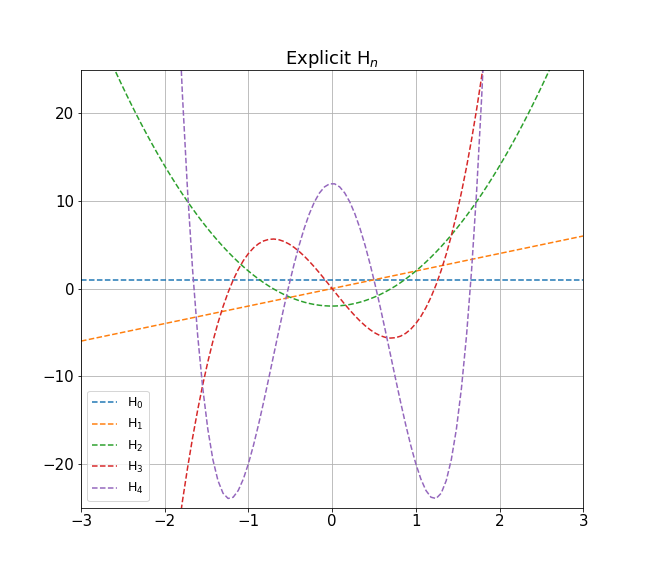
\includegraphics[scale = 0.4]{hexplicit}
  \caption{Hermite Polynomials: Explicit Method}
  \label{fig:hexp}
\end{figure}
For the indicated range, the numbers are sufficiently small that even a fourth power doesn't seem to alter the results that much. 
\vfill\eject
A recursion function was then used as another approach to generate the Hermite polynomials. Figure \ref{fig:hrec} shows the corresponding graph of this method.

\begin{figure}[h!]
  \centering
  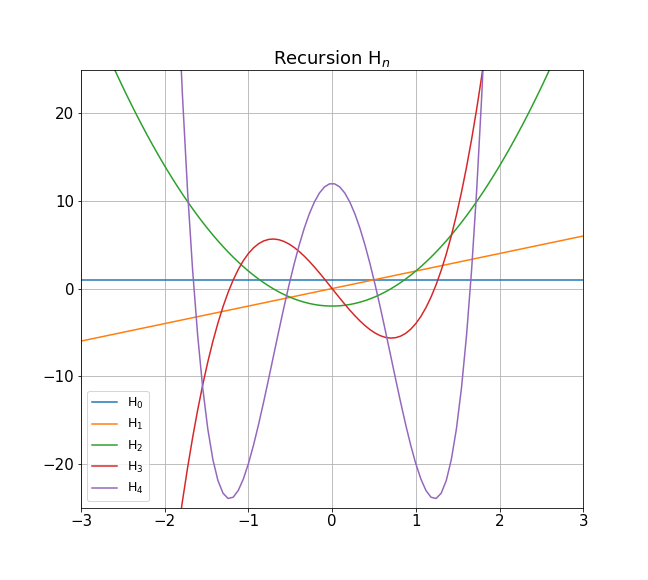
\includegraphics[scale = 0.4]{hrecursion}
  \caption{Hermite Polynomials: Recursion Method}
  \label{fig:hrec}
\end{figure}
To ensure that the mathematical expressions of the symbolic manipulation and the graphs were correct, Weissten's article on MathWorld was referenced. 
Figure \ref{fig:hwolf} shows the plot he provides.

\begin{figure}[h!]
  \centering
  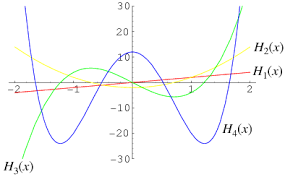
\includegraphics[scale = 0.4]{hwolfram}
  \caption{Hermite Polynomials \cite{weissteinH}}
  \label{fig:hwolf}
\end{figure}
Comparisons for $H_3$ and $H_4$ can be seen in Figures \ref{fig:h3} and \ref{fig:h4} accordingly. They are similar in value, and there does not seem to be any noticeable
difference between them. 

\begin{figure}[h]
  \centering
  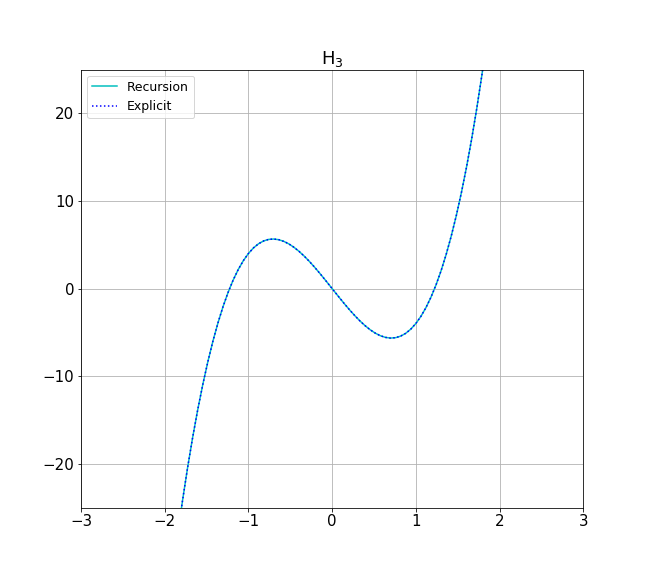
\includegraphics[scale = 0.4]{h3}
  \caption{Explicit and Recursion for $H_3$}
  \label{fig:h3}
\end{figure}

\begin{figure}[]
  \centering
  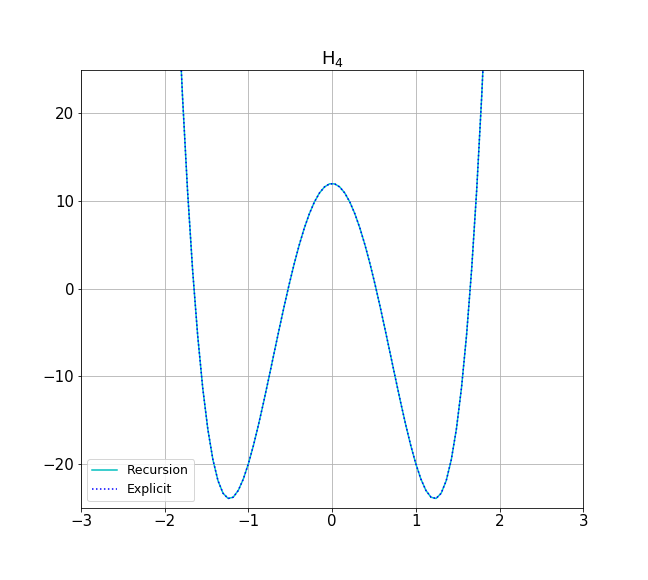
\includegraphics[scale = 0.4]{h4}
  \caption{Explicit and Recursion for $H_4$}
  \label{fig:h4}
\end{figure}
\vfill\eject
\section{Legendre Polynomials}
Using the provided recursion method for generating the Legendre Polynomials, plots were made for polynomials $P_0$ through $P_5$ and can be seen in Figure \ref{fig:leg}.

\begin{figure}[h]
  \centering
  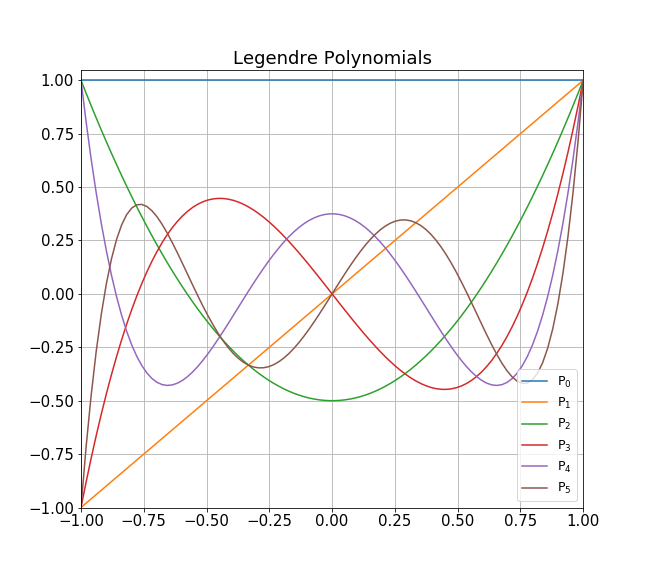
\includegraphics[scale = 0.4]{legendre}
  \caption{Legendre Polynomials}
  \label{fig:leg}
\end{figure}
For good measure, this was compared to Weissten's article about Legendre Polynomials, his plot shown in Figure \ref{fig:pwolf}.

\begin{figure}[h]
  \centering
  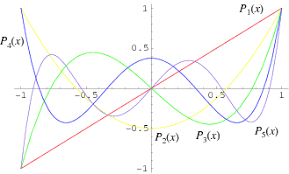
\includegraphics[scale = 0.4]{pwolfram}
  \caption{Legendre Polynomials \cite{weissteinP}}
  \label{fig:pwolf}
\end{figure}

\vfill\eject
\section{Numerical Derivatives}

Three methods were used to approximated derivatives for the function $f(x) = x^4$ at $x=10$. For the first derivative, 2-point and 4-point central finite
differences were used, and for the second derivative a 2-point difference was used.

To see the effects of different step-sizes $h$, 5 linearly spaced vectors were created with 2 orders of magnitude of difference between the boundries (ie 100 and 1). These
vectors where then stacked to define the interval for h, $h\in[10^2,10^{-8}]$.

Figures \ref{fig:df2p} through \ref{fig:d2f2p} accordingly represent the plot of the unsigned absolute error against the step-size for approximations of the derivatives.

The 2-point approximation for the first derivative can be seen in Figure \ref{fig:df2p}, andd seems to have best results when using step-sizes 
roughly between $10^{-5}$ and $10^{-4}$ orders of magnitude.
\begin{figure}[h!]
  \centering
  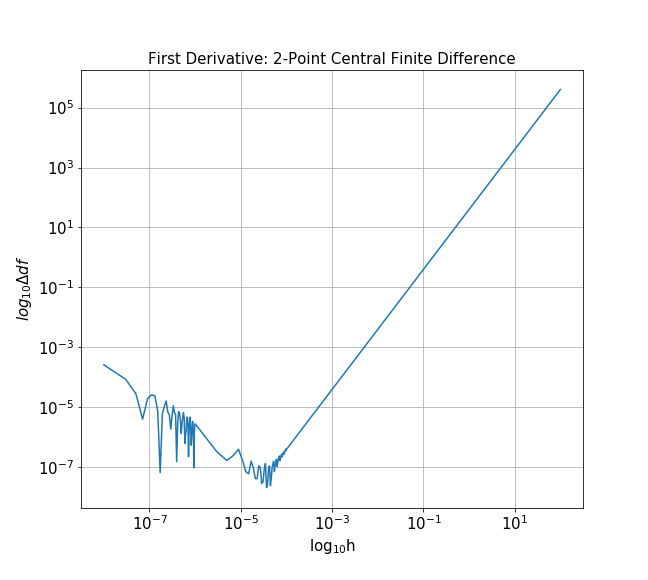
\includegraphics[scale = 0.4]{df2p}
  \caption{First Derivative: 2-Point Central Finite Difference}
  \label{fig:df2p}
\end{figure}
\vfill\eject
The 4-point approximation (Figure \ref{fig:df4p}) was much more volatile with its error, but its optimal values are seen in step-sizes between $10^{-1}$ and $10^{1}$.
\begin{figure}[h]
  \centering
  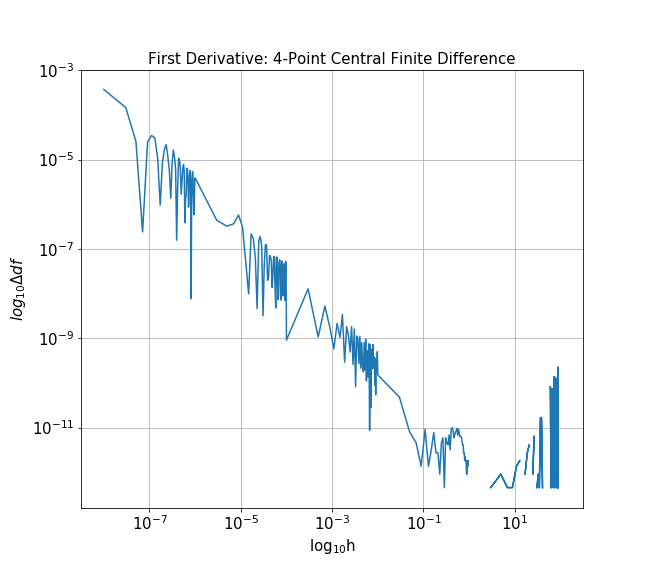
\includegraphics[scale = 0.4]{df4p}
  \caption{First Derivative: 4-Point Central Finite Difference}
  \label{fig:df4p}
\end{figure}

Figure \ref{fig:d2f2p} then shows the 2-point approximation for the second derivative of the function. Its minimal error can be seen when using a step-size of $10^{-3}$.
\begin{figure}[h!]
  \centering
  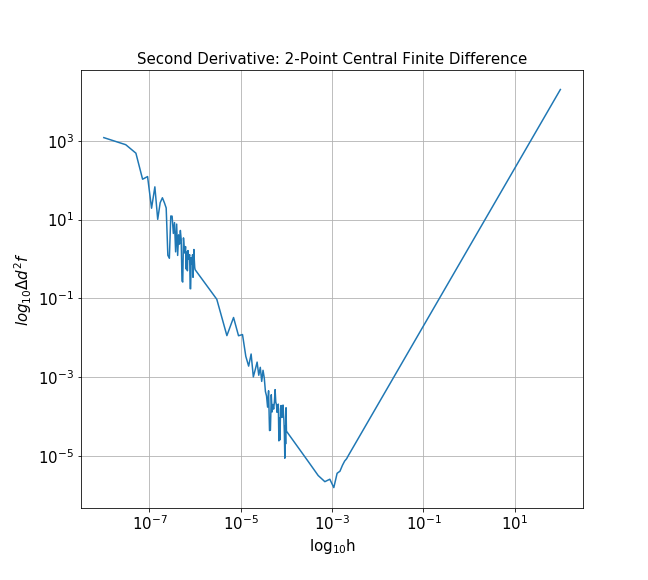
\includegraphics[scale = 0.4]{d2f2p}
  \caption{Second Derivative: 2-Point Central Finite Difference}
  \label{fig:d2f2p}
\end{figure}
\vfill\eject
\newpage
\bibliographystyle{apalike}
\addcontentsline{toc}{section}{References}
\bibliography{HW01}
\nocite{*}

\end{document}
